\documentclass[12pt, oneside]{article}
\usepackage{geometry}
\geometry{letterpaper}
\usepackage{graphicx}
\graphicspath{{images/}}
\usepackage{amsmath}
\usepackage{amsthm}	
\usepackage{amssymb}
\usepackage{diagbox}
\usepackage{hyperref}
\hypersetup{
	colorlinks=true,
	urlcolor=blue
}

\title{Math Journal}
\author{Andrew Ha}
\date{}								%no date

\newtheorem{proposition}{Proposition}
\newtheorem{identity}{Identity}

\begin{document}
\maketitle
\section*{Combinatorial Proof}
\textbf{09/10/2024}
\begin{proposition} For positive integers $n$ and $k$ with $n=2k, \frac{n!}{2!^k}$ is an integer. \end{proposition}
\emph{Proof.}  Consider the $n$ symbols: $x_1, x_1, x_2, x_2, \cdots, x_k, x_k$.
The number of arrangements of all these $n = 2k$ symbols is an integer that equals
\[
\frac{n!}{\underbrace{2! 2! \cdots 2!}_{\text{k factors of 2!}}} = \frac{n!}{2!^k}
\]
I learned this from the first day of class in MACM 101. This is an example of proving that a value is an integer by obtaining that value from counting something. Researching further, I also found out about double counting.\ It is based on the idea that counting the same objects in two different ways results in two different expressions, which must be equal to each other. 
\begin{identity} 
\[
2^n = \sum_{k=0}^{n}  \binom{n}{k}
\]
\end{identity}
For example, this identity can be proved by counting the number of subsets of a set $A$ with $n$ elements. One way to count this is noticing how you can either include or exclude each element, giving 2 choices for each of the $n$ elements. This gives $2^n$ subsets. Second way to count the number of subsets is summing up the number of subsets with $k$ elements where $k$ can be any integer from 0 to $n$. For each case, you would be choosing $k$ elements out of $n$ elements, so there are $\binom{n}{k}$ subsets.
Summing up, the total number of subsets is $\sum_{k=0}^{n}  \binom{n}{k}$.\ Two expressions, $2^n$ and $\sum_{k=0}^{n}  \binom{n}{k}$, must be equal since they represent the same thing.
\section*{Putnam 2002 B1}
\textbf{09/11/2024}
\\
\noindent Here is a fun problem I wanted to share from the 2002 William Lowell Putnam Mathematics Competition.
\begin{quote}
B1. Shanille O'Keal shoots free throws on a basketball court. She hits
the first and misses the second, and thereafter the probability that
she hits the next shot is equal to the proportion of shots she
has hit so far. What is the probability she hits exactly 50 of
her first 100 shots?
\end{quote}
This problem doesn't require much of advanced mathematics, yet it is simple and tricky. Here's a solution I like:\\

\emph{Solution.} The probability of $n$th success is the proportion of shots she has hit so far, which is $\frac{n - 1}{\text{\# of shots so far}}$. On the other hand, the probability of $n$th miss is $1 - \frac{\text{\# of successes so far}}{\text{\# of shots so far}} = \frac{\text{\# of shots so far}}{\text{\# of shots so far}} - \frac{\text{\# of shots so far} - (n - 1)}{\text{\# of shots so far}} = \frac{n-1}{\text{\# of shots so far}}$. For her to hit exactly 50 of her first 100 shots, she has to hit exactly 49 shots and miss exactly 49 shots. Consider the probability of one case where she hits 49 shots consecutively then misses 49 shots consecutively: 
\[
\underbrace{\frac{1}{2} \times \frac{2}{3} \times \frac{3}{4} \times \frac{4}{5} \times \cdots \times \frac{49}{50}}_\text{49 successes} \times \underbrace{\frac{1}{51} \times \frac{2}{52} \times \frac{3}{53} \times \frac{4}{54} \cdots \times \frac{49}{99}}_\text{49 misses} = \frac{49!^2}{99!}
\]
Here, the arrangement of shots does not affect the overall probability since the numerator will always be $49!^2$ as long as she hits 49 shots and misses 49 shots, and the denominator will always be 99!. Therefore, multiplying the probability of single case by the number of arrangements will give us the answer. The number of arrangements of 49 shots and 49 misses is $\frac{98!}{49!^2}$ since there are 49 duplicates of 2 cases. Multiplying two numbers yields
\[
\frac{49!^2}{99!} \cdot \frac{98!}{49!^2} = \frac{1}{99}
\]
The probability she hits exactly 50 of her first 100 shots is $\frac{1}{99}$.
\pagebreak
\section*{Two Random Distributions}
\textbf{09/16/2024}
\\
This is from a \href{https://www.youtube.com/watch?v=ga9Qk38FaHM}{YouTube video} I watched recently. It talks about a surprising fact that choosing a random number between 0 and 1 and calculating its square root is actually the same as choosing two random numbers between 0 and 1 and taking the larger one. To see why, we look at the distribution of two functions, max($X, Y$) and $\sqrt{X}$. $X$ and $Y$ are independent and random numbers between 0 and 1. Since two distributions are continuous, the probability of getting a specific number is 0. Instead, we look at the probability of getting a number less than or equal to $n$. For max($X, Y$), both $X$ and $Y$ must be less than or equal to $n$. Notice that the probability of getting a number less than or equal to $n$ is $n$ since it is between 0 and 1.
\[
P(\text{max}(X, Y) \leq n) = P(X \leq n) \cdot P(Y \leq n) = n^2
\]
Now, for $\sqrt{X}$, $X$ has to be less than or equal to $n^2$ for $\sqrt{X}$ to be less than or equal to $n$.
\[
P(\sqrt{X} \leq n) = P(X \leq n^2) = n^2
\]
This can actually be generalized that choosing a max value of $m$ random numbers between 0 and 1 and taking the $m$th root of a random number between 0 and 1 are identical. 
\begin{eqnarray*}
P(\text{max}(X_1, X_2, \cdots, X_m) \leq n) = & P(X_1 \leq n) P(X_2 \leq n) \cdots P(X_m \leq n) & = n^m\\
P(\sqrt[m]{X} \leq n) = & P(X \leq n^m) & = n^m
\end{eqnarray*}
This reminds me of what I learned in statistics about probabilities.
\section*{$\bigwedge$}
\textbf{09/17/2024}\\
I had a funny thought while walking to school today. I imagined two bicycles coming from opposite sides of a road that narrows suddenly in the middle of them. There would be two types of people, people who slow down for the other person to pass first (call them D) and people who speed up to pass faster than the other person (call them U). If D and D meet, or if U and D meet, there will be no accident. However, if U and U meet, there will be an accident. I thought of the truth table for AND ($\wedge$).
\begin{center}
\begin{tabular} {| c | c | c |}
\hline
$p$ & $q$ & $p \wedge q$\\
\hline
T & T & T\\
\hline
T & F & F\\
\hline
F & T & F\\
\hline
F & F & F\\
\hline
\end{tabular}
\end{center}
Asking "accident?", D say no (F), and U say yes (T). Two meeting in the road is the AND operation, so the result comes out as the truth table suggests.
\section*{Intro Puzzle from Jane Street}
\textbf{09/21/2024}\\
Last school year, I got an email from the Mathematical Association of America leading me to the \href{https://www.janestreet.com/puzzles/}{puzzles page} in Jane Street. This is the intro puzzle:
\begin{quote}
\textbf{Why Puzzles}

What’s a company like Jane Street doing with a page about puzzles? The act of solving puzzles, though that might seem abstract, is intrinsic to the work we do at Jane Street.

Only by identifying new problems in the financial markets and figuring out (potentially novel) ways to solve them can Jane Street continue to thrive. Even though we have established strategies, we’re humble enough to know that if we have a good idea, others may soon have it as well. Prime among the skills necessary to stay successful, then, is creative problem solving, or puzzling.

Number puzzles, logic puzzles, puzzles with and without clear answers, puzzles with and without clearly defined rules — these are all part of day-to-day life at Jane Street, which is why we’ve chosen to devote this section of our website to puzzles. Plus, solving puzzles just feels great.

One last thing — this is a puzzle!
\end{quote}
At first, I spent about 30 minutes just staring at the text.\ Eventually I found the way to decode it; I just needed to look at the capitalized words. Bringing out all the capitalized words, it reads "What's The Only Even Prime Number Plus One", so the answer is $2+1=3$.

Jane Street has been positng a puzzle every month since 2014, and some are challenging while some are doable (especially the older ones). I tried the \href{https://www.janestreet.com/puzzles/hooks-index/}{second oldest puzzle} where you need to enter nine 9’s in the outermost hook, eight 8’s in the next hook, then seven 7’s, six 6’s, and so on, down to the one 1 (already entered), so that the row and column sums match the values given along the border.\\
\begin{center}
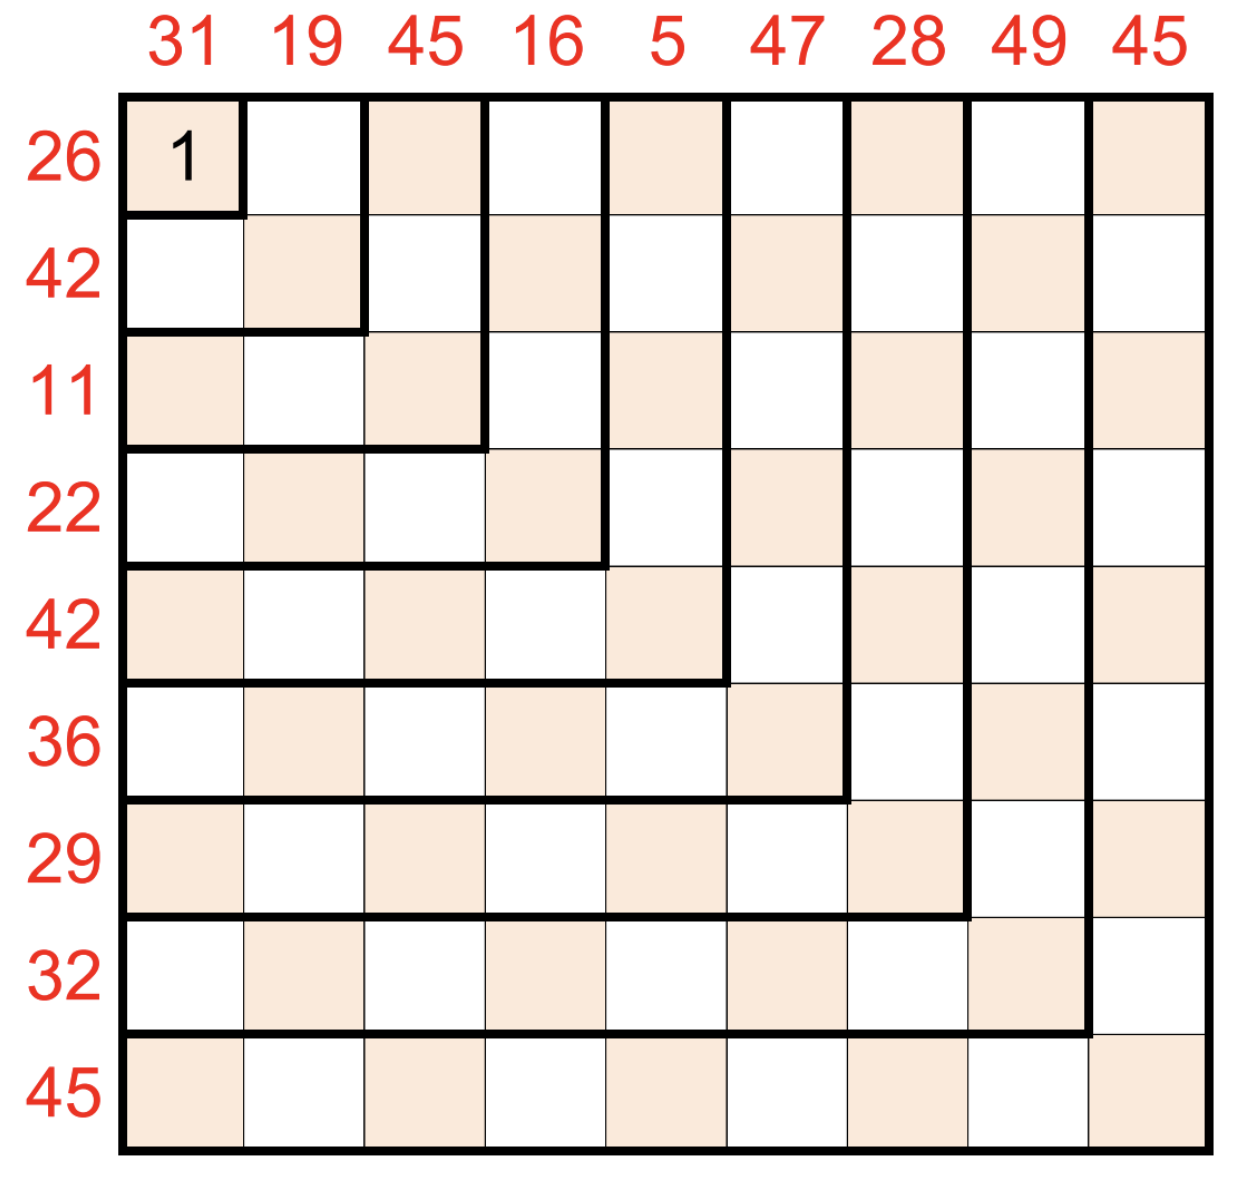
\includegraphics[scale=0.4]{puzzle1}
\end{center}
It was easy to solve given enough time because I could fill out the grid from the bottom right corner one by one. I figured that it would be easy to manipulate the answer (eg.\ add/multiply certain squares) so I can get the number I want with  puzzles similar to this.
\section*{A Counting Problem}
\textbf{09/23/2024}\\
This is a counting problem I struggled to solve without any hints. 
\begin{quote}
For $n \geq 4$, consider the strings made up of $n$ bits --- that is, a total of n 0's and 1's. In particular, consider those strings where there are (exactly) two occurrences of 01. How many such strings are there?
\end{quote}
I wrote down the small cases to find a pattern. 
\begin{center}
\begin{tabular} {|c|c|c|c|c|}
\hline
 \diagbox{$n$}{\# of 01} & \textbf{0} & \textbf{1} & \textbf{2} & \textbf{3}\\
 \hline
 \textbf{4} & 5 & 10 & 1 & 0\\
 \hline
 \textbf{5} & 6 & 20 & 6 & 0\\
 \hline
 \textbf{6} & 7 & 35 & 21 & 1\\
 \hline
 \textbf{7} & 8 & 56 & 56 & 8\\
 \hline
\end{tabular}
\end{center}
I counted the small cases with hand, and I used that the sum of the numbers in a row must add up to $2^n$ to fill the rest of the table. After completing the third row, I noticed that all the numbers in $n$th row are from $(n+1)$th row of Pascal's triangle, so I used this fact to complete the fourth row. I eventually guessed the formula for the number of binary strings of length $n$ with $k$ 01s to be $\binom{n+1}{2k+1}$. However, I could not figure out how choosing $2k+1$ out of $n+1$ objects can represent a binary string of length $n$ with $k$ 01s. I examined the specific case of $n=6$, $k=2$ and $\binom{n+1}{2k+1} = \binom{7}{5}$. I counted how many times 0 switches to 1 or 1 to 0 for the string to have 2 occurrences of 01, and there were 4 cases if I shortened any repeating digits to just one of them. \\

\begin{tabular}{c l l}
1) & 0101 & Switches 3 times\\
2) & 01010 & Switches 4 times\\
3) & 10101 & Switches 4 times\\
4) & 101010 & Switches 5 times\\
\end{tabular}\\

\noindent I realized that you can merge all four cases by putting 1 at the front and 0 at the end.\\

\begin{tabular}{c l c l}
1) & 0101 & $\rightarrow$ & 101010\\
2) & 01010 & $\rightarrow$ & 101010\\
3) & 10101 & $\rightarrow$ & 101010\\
4) & 101010 & $\rightarrow$ & 101010\\
\end{tabular}\\

\noindent With extra 1 and 0, there are now 8 letters and thus 7 places (between each letter) where 0 and 1 can be switched, and they are always switched 5 times. We now choose 5 out of 7 places to have exactly 2 occurrences of 01, so we obtain the desired number, $\binom{7}{5}$. To generalize, there are $\binom{n+1}{2k+1}$ strings with exactly $k$ occurrences of 01 and length $n$. Thus, the answer we are looking for is $\binom{n+1}{5}$.
\section*{Putnam 2013 A1}
\textbf{09/24/2023}\\
Here's another simple problem from the Putnam competition. 
\begin{quote}
Recall that a regular icosahedron is a convex polyhedron having 12 vertices and 20 faces; the faces are congruent equilateral triangles. On each face of a regular
icosahedron is written a nonnegative integer such that
the sum of all 20 integers is 39. Show that there are
two faces that share a vertex and have the same integer
written on them.
\end{quote}
When I tried this problem, I tried to figure out the maximum number of same integer that can be written by drawing out the icosahedron and trying to put in single number as many as possible. I was able to put 4 without a sharing vertex, but I wasn't able to find a way to put 5. I figured 4 was the maximum although I couldn't think of a way to prove it. To minimize the sum, I needed to put 5 smallest nonnegative integers (0, 1, 2, 3, 4) 4 times each which gives the sum of $4 \cdot (0 + 1 + 2 + 3 + 4) = 40$. Thus, the sum of 39 cannot be achieved without two faces sharing a vertex and having the same integer written on them. This solution is valid if I could prove that 4 is the maximum number of same integer that can be written.

It turned out that there was a simple and beautiful proof for it. If the same integer is written on 5 different triangular faces, and none of the vertices are shared, then there are 15 different vertices in an icosahedron. Since there are only 12 vertices in an icosahedron,  the maximum number of same integer that can be written is 4.
\end{document}